%%%%%%%%%%%%%%%%%%%%%%%%%%%%%%%%%%%%%%%%%
% University/School Laboratory Report
% LaTeX Template
% Version 3.1 (25/3/14)
%
% This template has been downloaded from:
% http://www.LaTeXTemplates.com
%
% Original author:
% Linux and Unix Users Group at Virginia Tech Wiki 
% (https://vtluug.org/wiki/Example_LaTeX_chem_lab_report)
%
% License:
% CC BY-NC-SA 3.0 (http://creativecommons.org/licenses/by-nc-sa/3.0/)
%
%%%%%%%%%%%%%%%%%%%%%%%%%%%%%%%%%%%%%%%%%

%----------------------------------------------------------------------------------------
%	PACKAGES AND DOCUMENT CONFIGURATIONS
%----------------------------------------------------------------------------------------

\documentclass{article}

\usepackage[version=3]{mhchem} % Package for chemical equation typesetting
\usepackage{siunitx} % Provides the \SI{}{} and \si{} command for typesetting SI units
\usepackage{graphicx} % Required for the inclusion of images
\usepackage{natbib} % Required to change bibliography style to APA
\usepackage{amsmath} % Required for some math elements 

\setlength\parindent{0pt} % Removes all indentation from paragraphs

\renewcommand{\labelenumi}{\alph{enumi}.} % Make numbering in the enumerate environment by letter rather than number (e.g. section 6)

%\usepackage{times} % Uncomment to use the Times New Roman font

%----------------------------------------------------------------------------------------
%	DOCUMENT INFORMATION
%----------------------------------------------------------------------------------------

\title{Lab Report 3 \\ Multiplexer and Decoder \\ ECE 238L \\} % Title
\author{Kenneth Cox}
\date{\today} % Date for the report

\begin{document}

\maketitle % Insert the title, author and date

\begin{center}
\begin{tabular}{l r}
Date Performed: & Mar 26, 2021 \\ % Date the experiment was performed
Instructor: & Professor Hamke % Instructor/supervisor
\end{tabular}
\end{center}

% If you wish to include an abstract, uncomment the lines below
% \begin{abstract}
% Abstract text
% \end{abstract}

%----------------------------------------------------------------------------------------
%	SECTION 1
%----------------------------------------------------------------------------------------


% If you have more than one objective, uncomment the below:
%\begin{description}
%\item[First Objective] \hfill \\
%Objective 1 text
%\item[Second Objective] \hfill \\
%Objective 2 text
%\end{description}

\section{Items}

\begin{description}
\item[Gates]
\item[Multiplexer]
\item[7 Segment Display]
\item[Top Level Module]
\end{description} 
 
%----------------------------------------------------------------------------------------
%	SECTION 2
%----------------------------------------------------------------------------------------


\begin{figure}[h]
\begin{center}
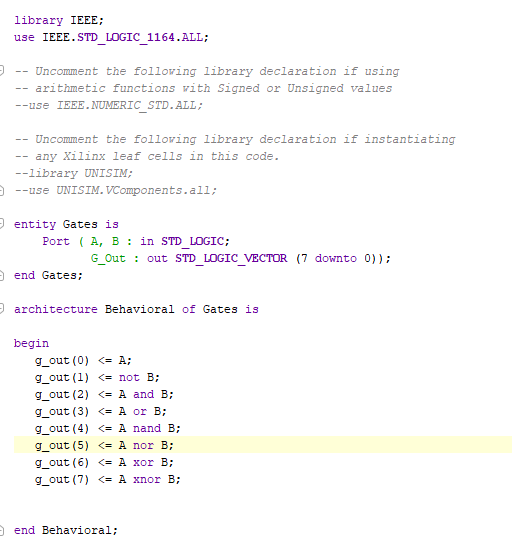
\includegraphics[width=1\textwidth]{GatesSource.png} % Include the image placeholder.png
\caption{source}
\end{center}
\end{figure}

\begin{figure}[h]
\begin{center}
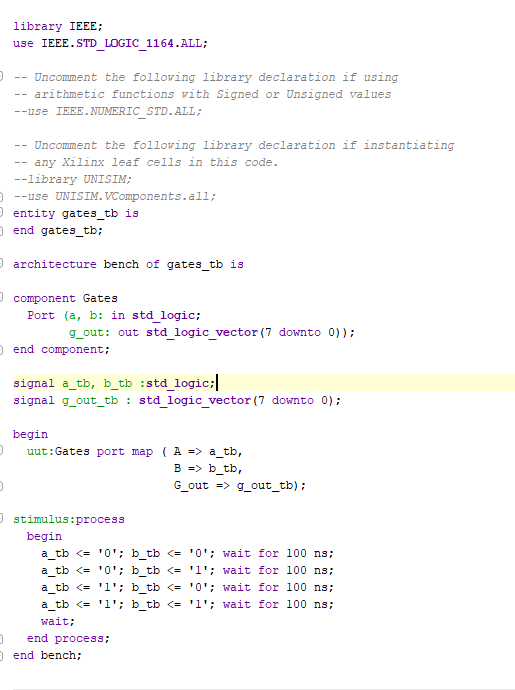
\includegraphics[width=1\textwidth]{GatesTestSource.png} % Include the image placeholder.png
\caption{test bench}
\end{center}
\end{figure}

\begin{figure}[h]
\begin{center}
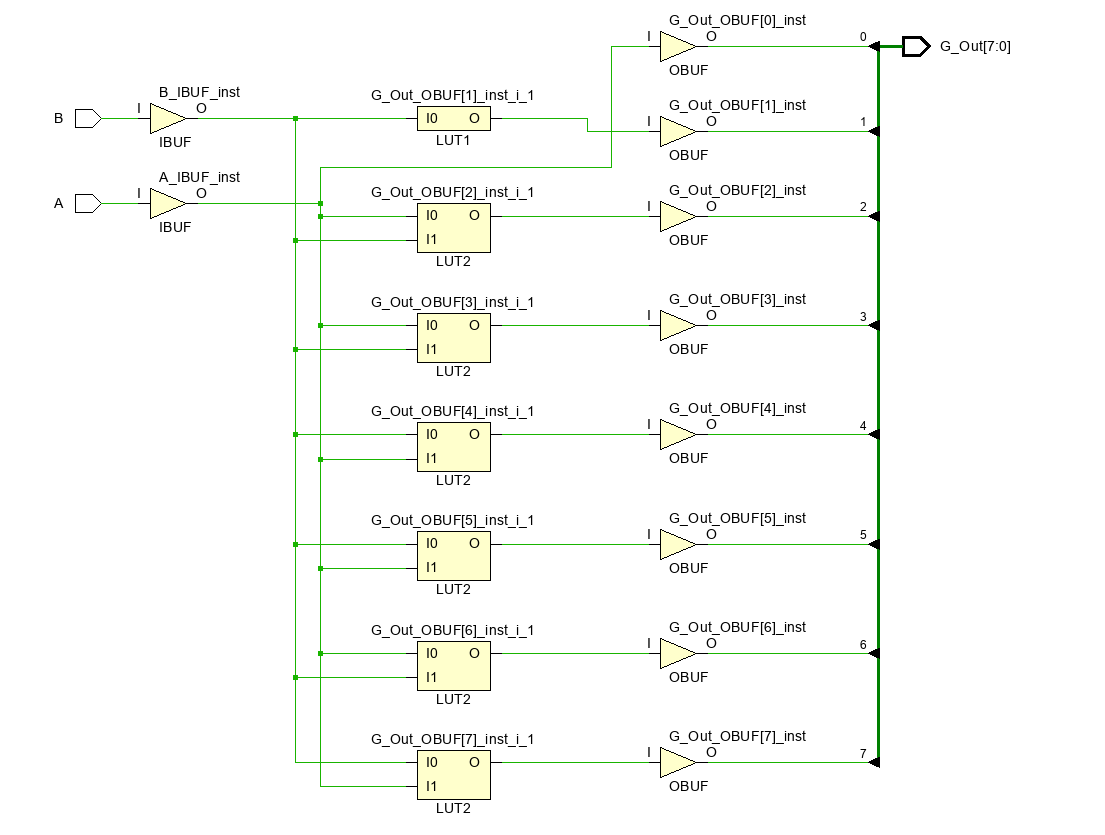
\includegraphics[width=1\textwidth]{GatesSchematic.png} % Include the image placeholder.png
\caption{Schematic}
\end{center}
\end{figure}


\begin{figure}[h]
\begin{center}
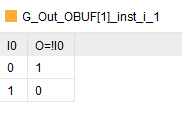
\includegraphics[width=1\textwidth]{GatesTruthTable.png} % Include the image placeholder.png
\caption{Truth Table}
\end{center}
\end{figure}


\begin{figure}[h]
\begin{center}
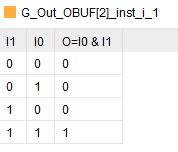
\includegraphics[width=1\textwidth]{GatesTruthTableCont.png} % Include the image placeholder.png
\caption{Truth Table}
\end{center}
\end{figure}


\begin{figure}[h]
\begin{center}
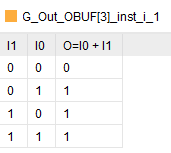
\includegraphics[width=1\textwidth]{GatesTruthTableCont1.png} % Include the image placeholder.png
\caption{Truth Table}
\end{center}
\end{figure}

\begin{figure}[h]
\begin{center}
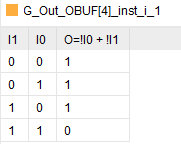
\includegraphics[width=1\textwidth]{GatesTruthTableCont2.png} % Include the image placeholder.png
\caption{Truth Table}
\end{center}
\end{figure}


\begin{figure}[h]
\begin{center}
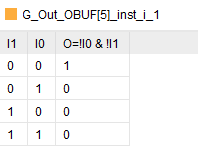
\includegraphics[width=1\textwidth]{GatesTruthTableCont3.png} % Include the image placeholder.png
\caption{Truth Table}
\end{center}
\end{figure}

\begin{figure}[h]
\begin{center}
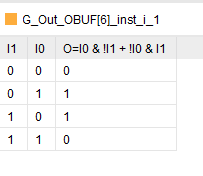
\includegraphics[width=1\textwidth]{GatesTruthTableCont4.png} % Include the image placeholder.png
\caption{Truth Table}
\end{center}
\end{figure}

\begin{figure}[h]
\begin{center}
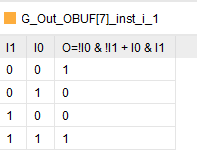
\includegraphics[width=1\textwidth]{GatesTruthTableCont6.png} % Include the image placeholder.png
\caption{Truth Table}
\end{center}
\end{figure}

\begin{figure}[h]
\begin{center}
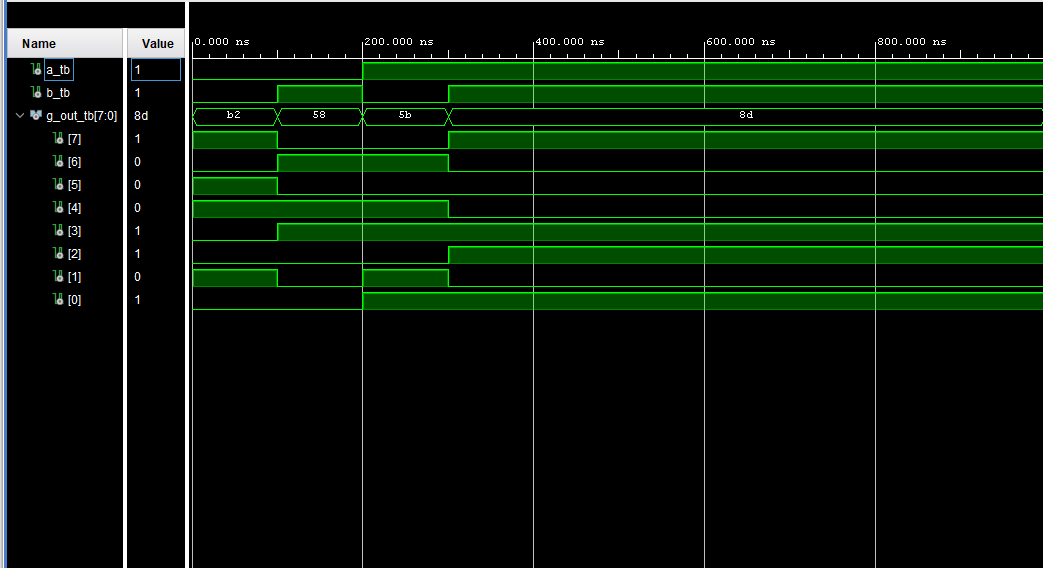
\includegraphics[width=1\textwidth]{GatesWaveForm.png} % Include the image placeholder.png
\caption{Truth Table}
\end{center}
\end{figure}
%----------------------------------------------------------------------------------------
%	SECTION 3
%----------------------------------------------------------------------------------------

\begin{figure}[h]
\begin{center}
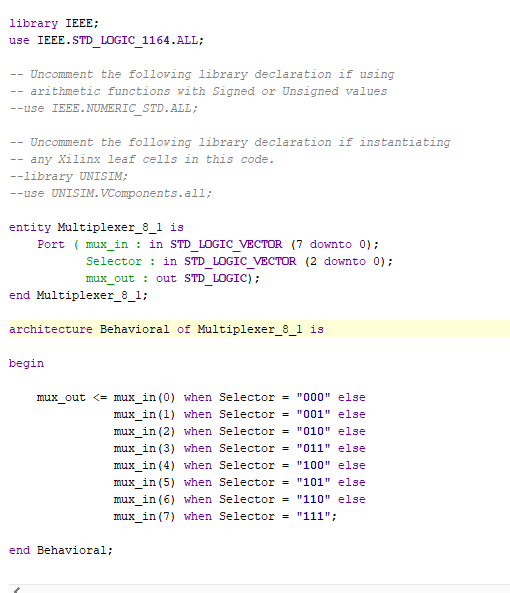
\includegraphics[width=1\textwidth]{MultiplexerSource.png} % Include the image placeholder.png
\caption{source}
\end{center}
\end{figure}

\begin{figure}[h]
\begin{center}
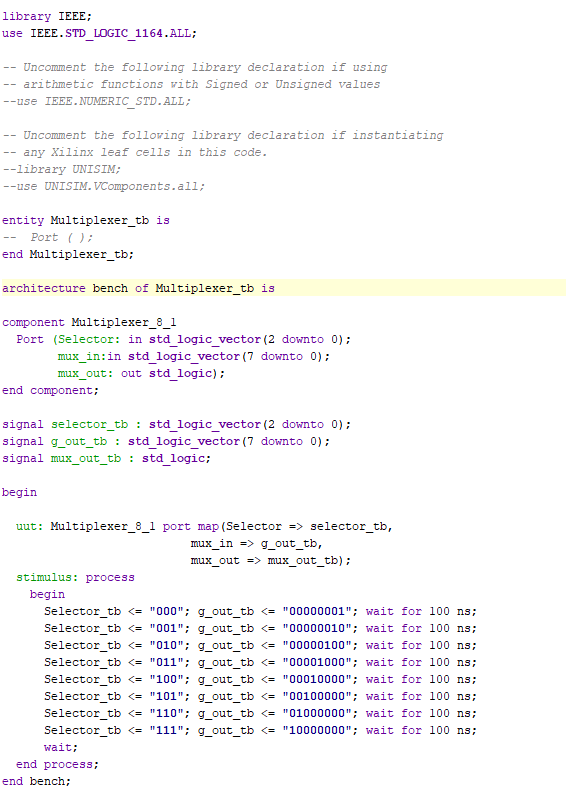
\includegraphics[width=1\textwidth]{MultiplexerTestSource.png} % Include the image placeholder.png
\caption{test bench}
\end{center}
\end{figure}

\begin{figure}[h]
\begin{center}
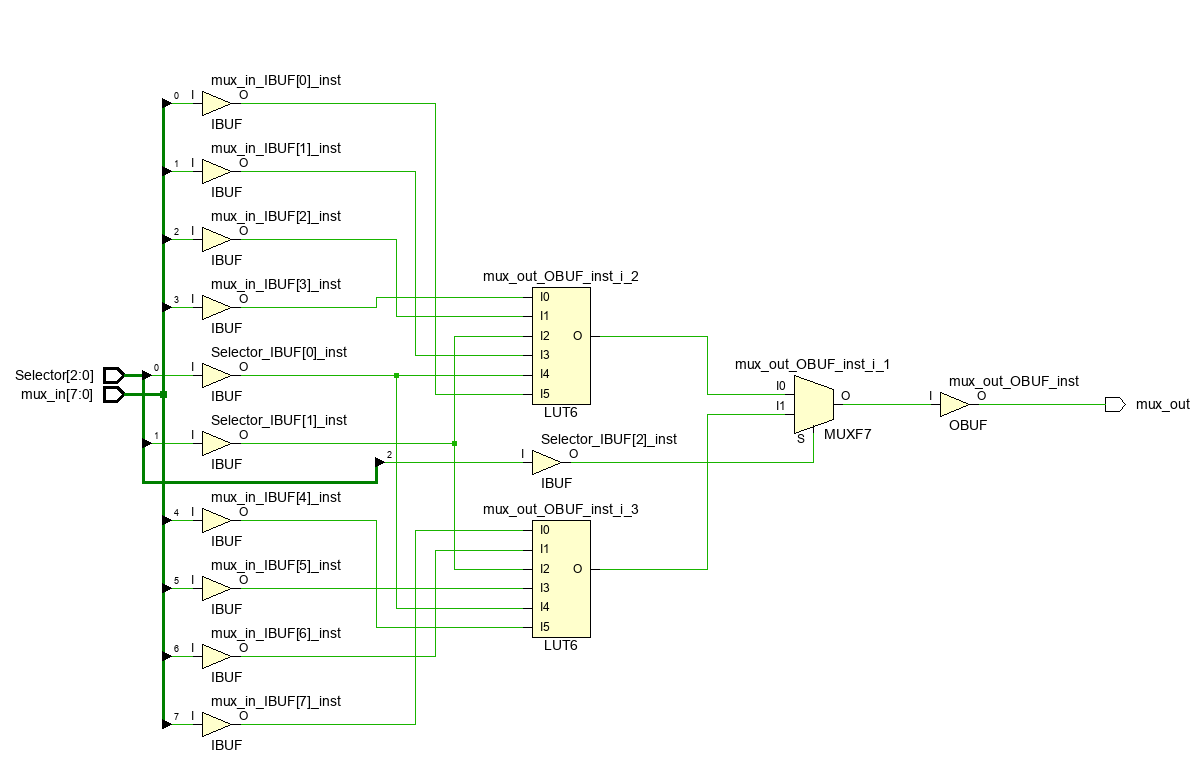
\includegraphics[width=1\textwidth]{MultiplexerSchematic.png} % Include the image placeholder.png
\caption{Schematic}
\end{center}
\end{figure}


\begin{figure}[h]
\begin{center}
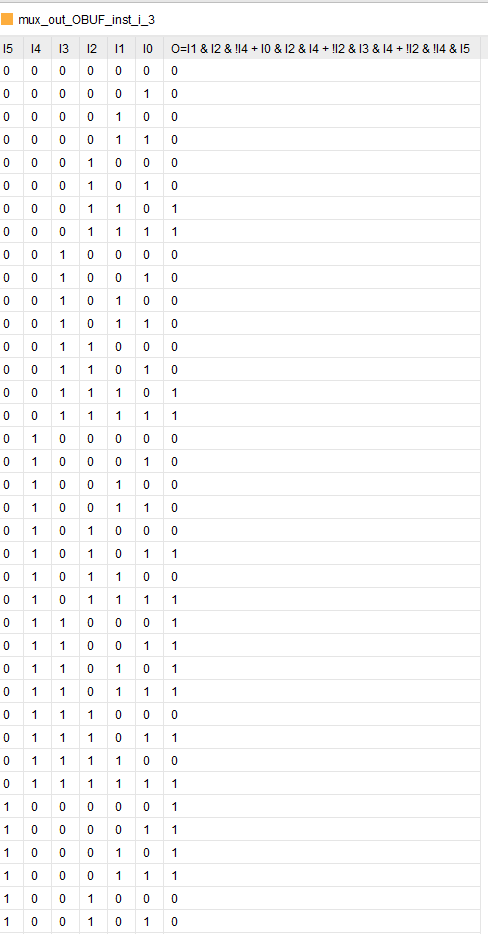
\includegraphics[width=1\textwidth]{MultiplexerTruthTable.png} % Include the image placeholder.png
\caption{Truth Table}
\end{center}
\end{figure}


\begin{figure}[h]
\begin{center}
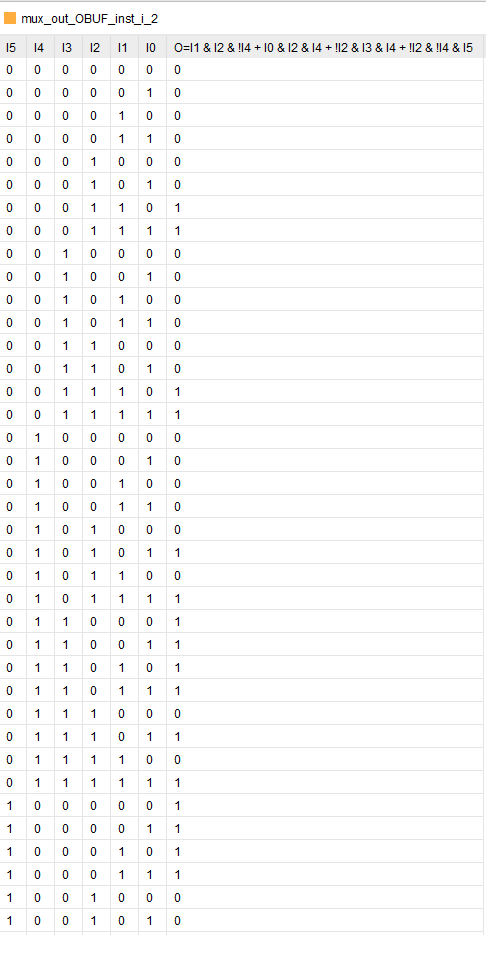
\includegraphics[width=1\textwidth]{MultiplexerTruthTableCont.png} % Include the image placeholder.png
\caption{Truth Table cont.}
\end{center}
\end{figure}


\begin{figure}[h]
\begin{center}
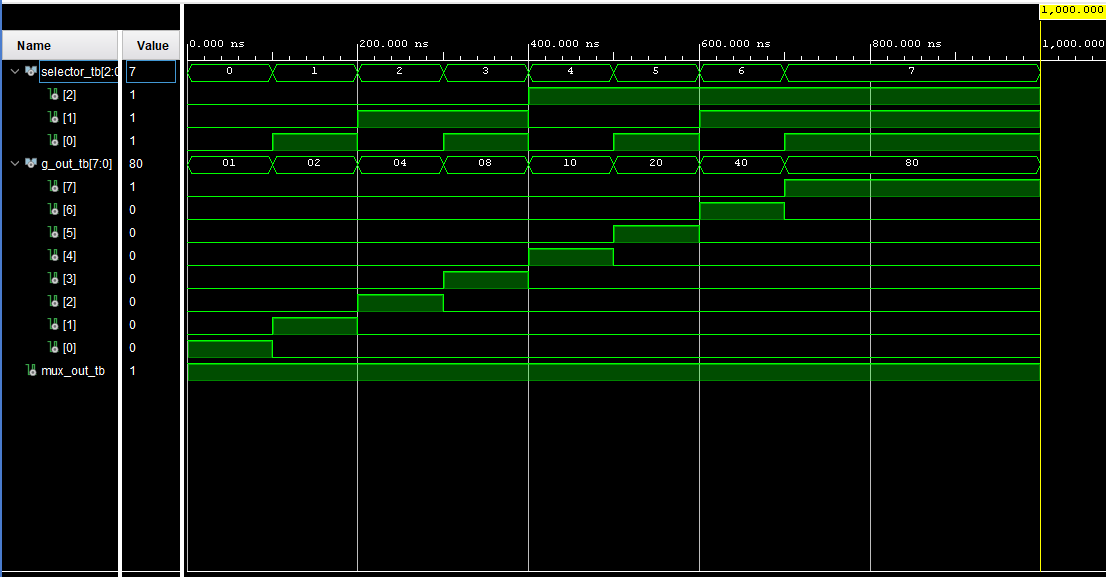
\includegraphics[width=1\textwidth]{MultiplexerWaveForm.png} % Include the image placeholder.png
\caption{Waveform}
\end{center}
\end{figure}

%----------------------------------------------------------------------------------------
%	SECTION 4
%----------------------------------------------------------------------------------------


\begin{figure}[h]
\begin{center}
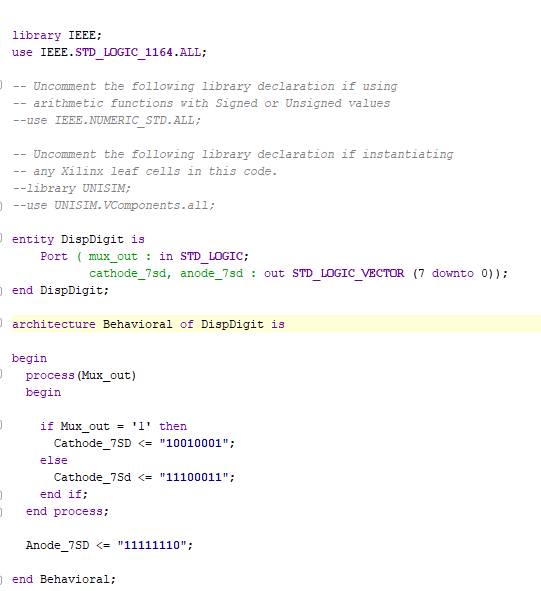
\includegraphics[width=1\textwidth]{DisplaySource.png} % Include the image placeholder.png
\caption{source}
\end{center}
\end{figure}

\begin{figure}[h]
\begin{center}
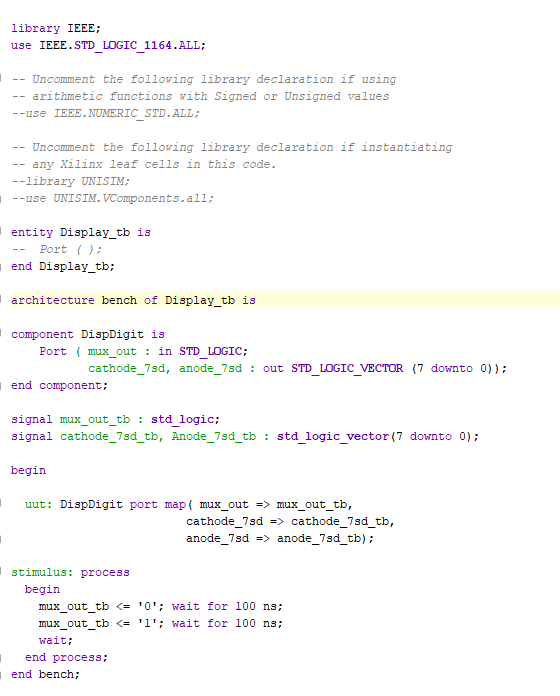
\includegraphics[width=1\textwidth]{DisplayTestSource.png} % Include the image placeholder.png
\caption{test bench}
\end{center}
\end{figure}

\begin{figure}[h]
\begin{center}
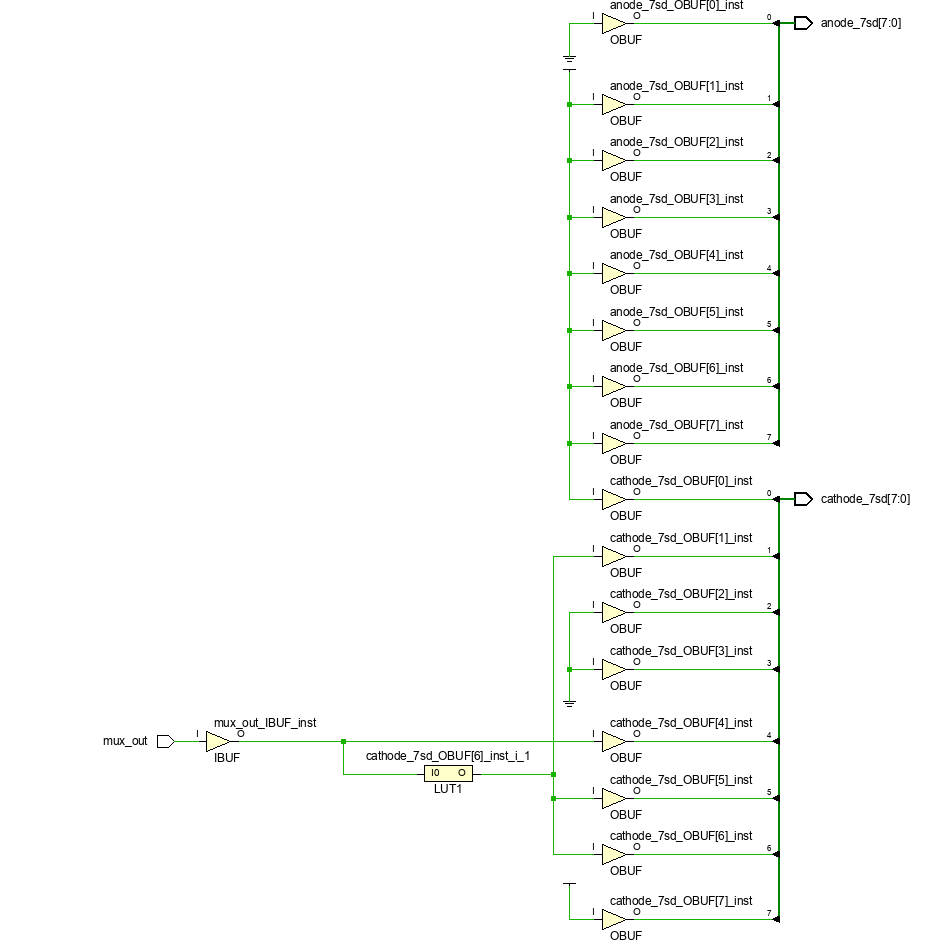
\includegraphics[width=1\textwidth]{DisplaySchematic.png} % Include the image placeholder.png
\caption{Schematic}
\end{center}
\end{figure}


\begin{figure}[h]
\begin{center}
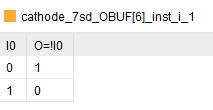
\includegraphics[width=1\textwidth]{DisplayTruthTable.png} % Include the image placeholder.png
\caption{Truth Table}
\end{center}
\end{figure}


\begin{figure}[h]
\begin{center}
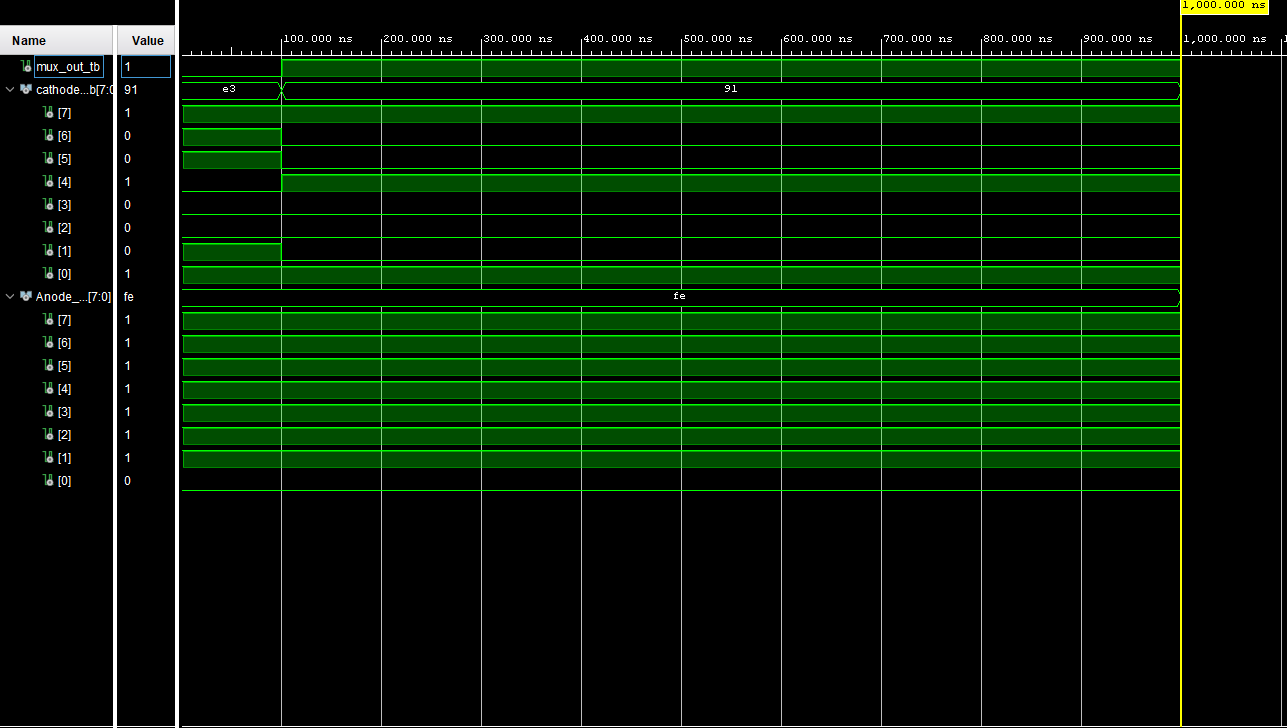
\includegraphics[width=1\textwidth]{DisplayWaveForm.png} % Include the image placeholder.png
\caption{Wavefrom}
\end{center}
\end{figure}


%----------------------------------------------------------------------------------------
%	SECTION 5
%----------------------------------------------------------------------------------------


\begin{figure}[h]
\begin{center}
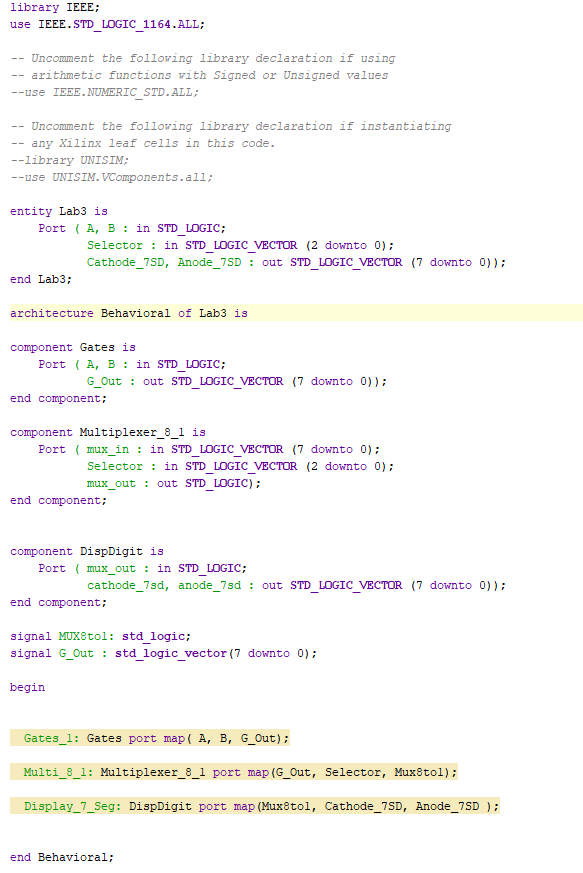
\includegraphics[width=1\textwidth]{DecoderSource.png} % Include the image placeholder.png
\caption{source}
\end{center}
\end{figure}

\begin{figure}[h]
\begin{center}
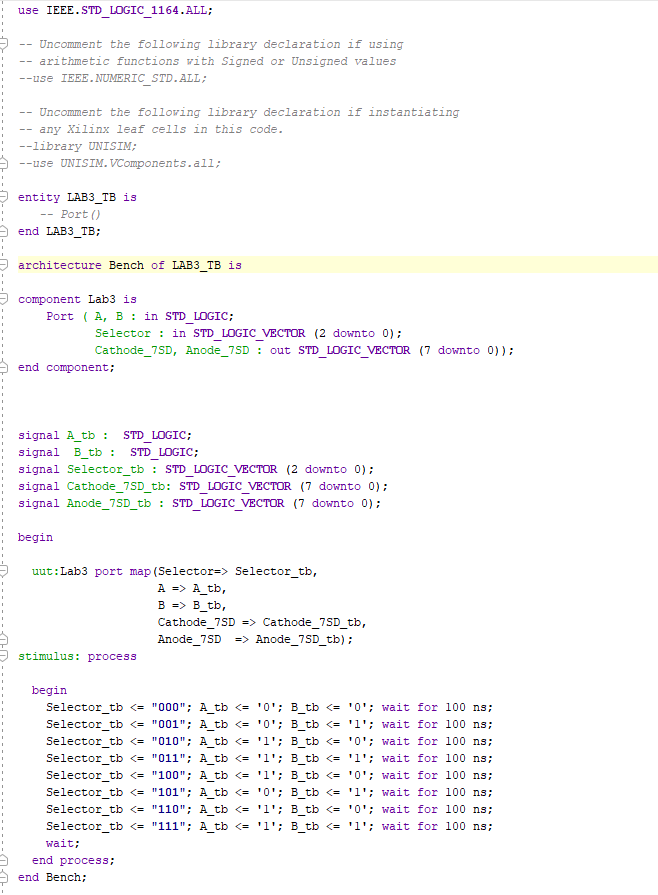
\includegraphics[width=1\textwidth]{DecoderTestSource.png} % Include the image placeholder.png
\caption{test bench}
\end{center}
\end{figure}

\begin{figure}[h]
\begin{center}
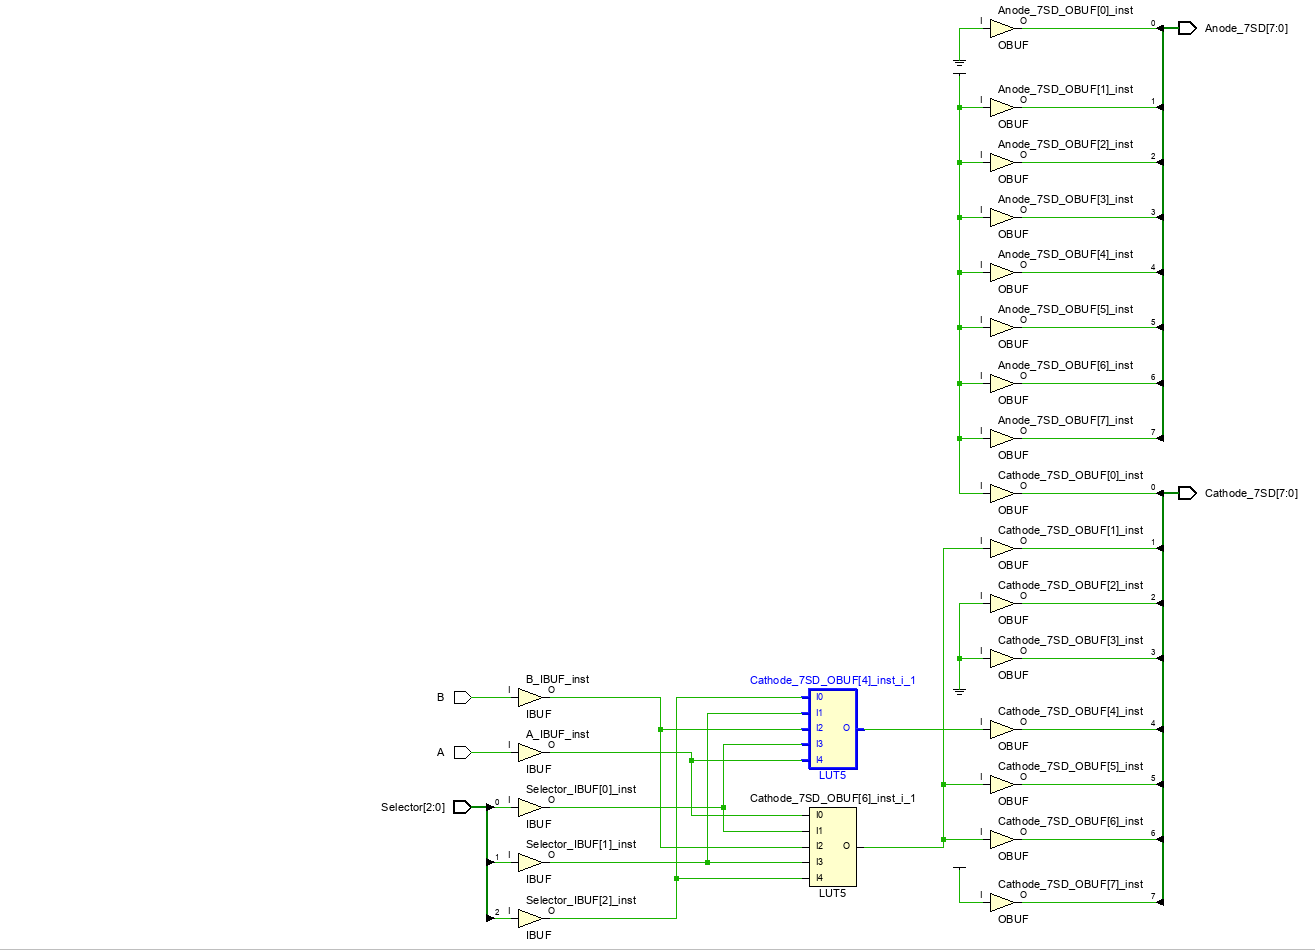
\includegraphics[width=1\textwidth]{DecoderSchematic.png} % Include the image placeholder.png
\caption{Schematic}
\end{center}
\end{figure}


\begin{figure}[h]
\begin{center}
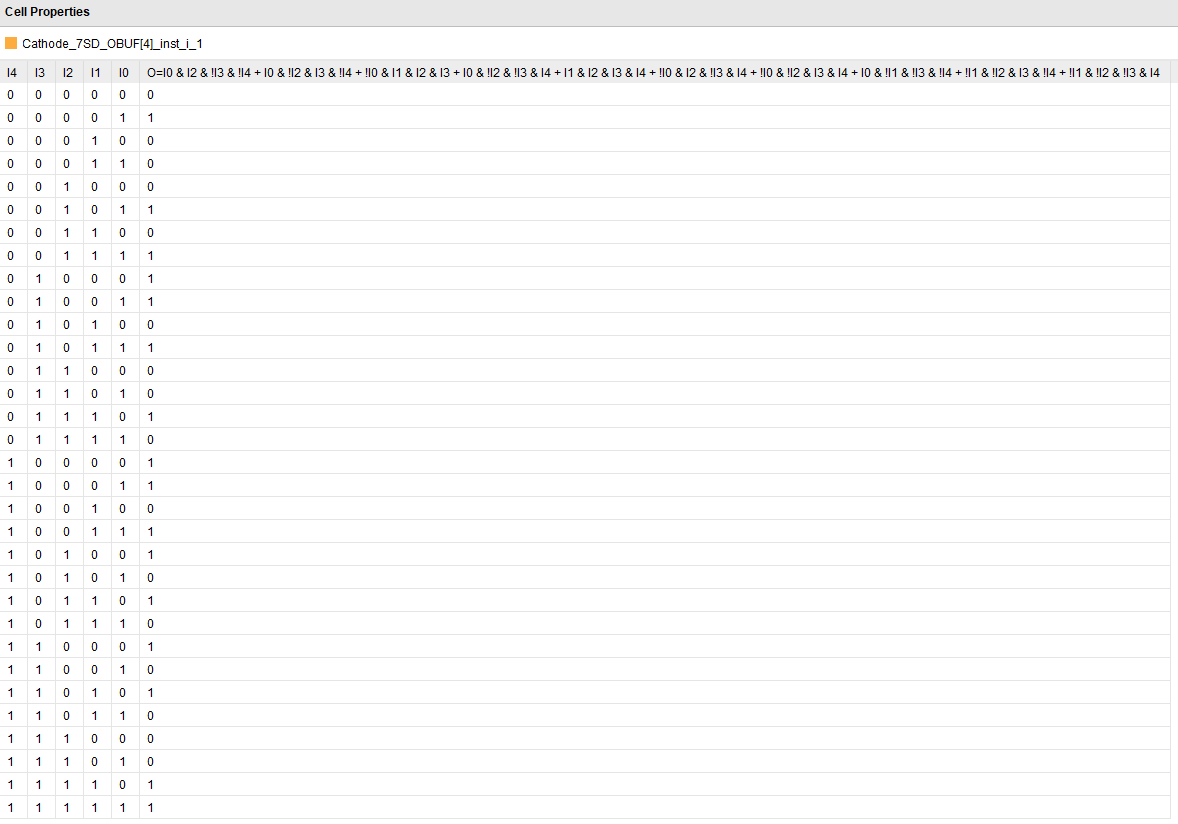
\includegraphics[width=1\textwidth]{DecoderTruthTable.png} % Include the image placeholder.png
\caption{Truth Table}
\end{center}
\end{figure}


\begin{figure}[h]
\begin{center}
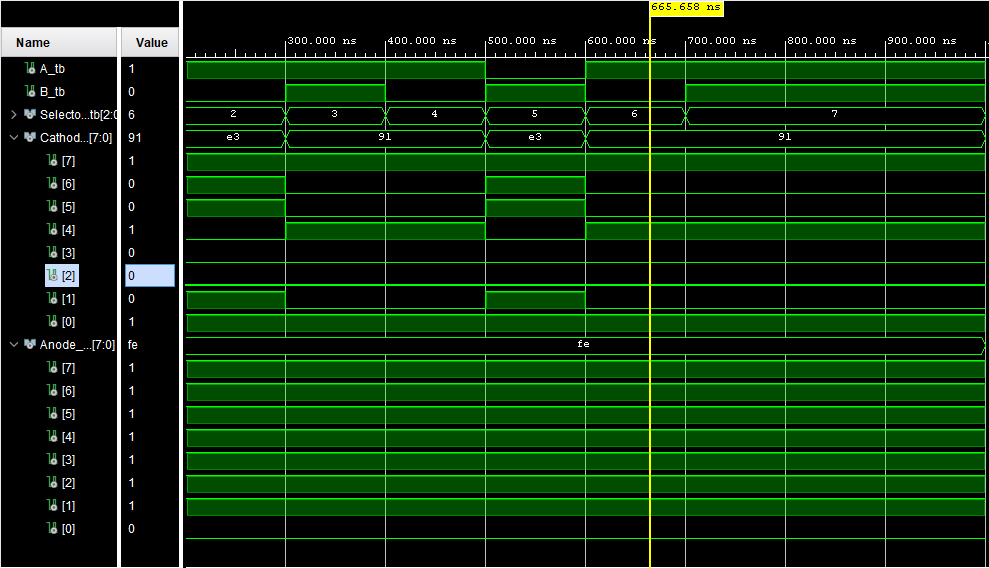
\includegraphics[width=1\textwidth]{DecoderWaveForm.png} % Include the image placeholder.png
\caption{Decoder Wave}
\end{center}
\end{figure} 
%----------------------------------------------------------------------------------------
%	SECTION 6
%----------------------------------------------------------------------------------------

\section{Feedback}
Initially, on my first attempt at this lab it was, at least the Decoder, somewhat confusing.


%----------------------------------------------------------------------------------------
%	BIBLIOGRAPHY
%----------------------------------------------------------------------------------------

\bibliographystyle{apalike}

\bibliography{sample}

%----------------------------------------------------------------------------------------


\end{document}